\begin{scanpage}{0126}{109}
\noindent\begin{minipage}[t]{.48\linewidth}\vspace{0pt}\centering
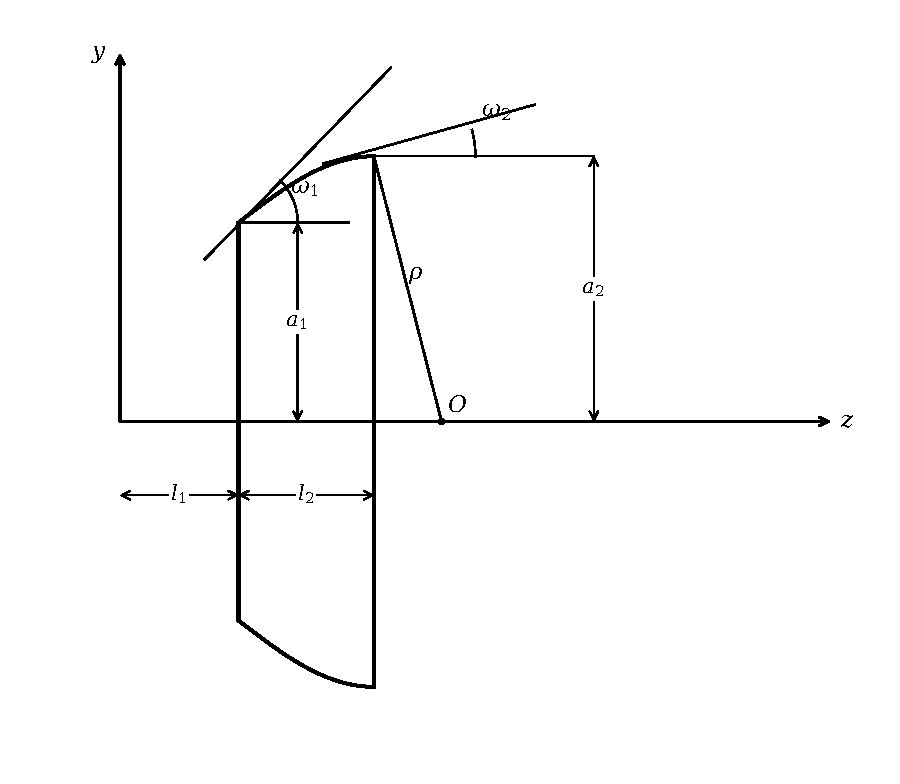
\includegraphics[width=.8\linewidth]{images/recreated/b-0126-fig41.pdf}

\raggedright Figure 41. A ring cut from the surface of its sphere by the planes $z=l_1$ and $z=l_1+l_2$.
\end{minipage}\hfill\begin{minipage}[t]{.48\linewidth}\vspace{0pt}\centering
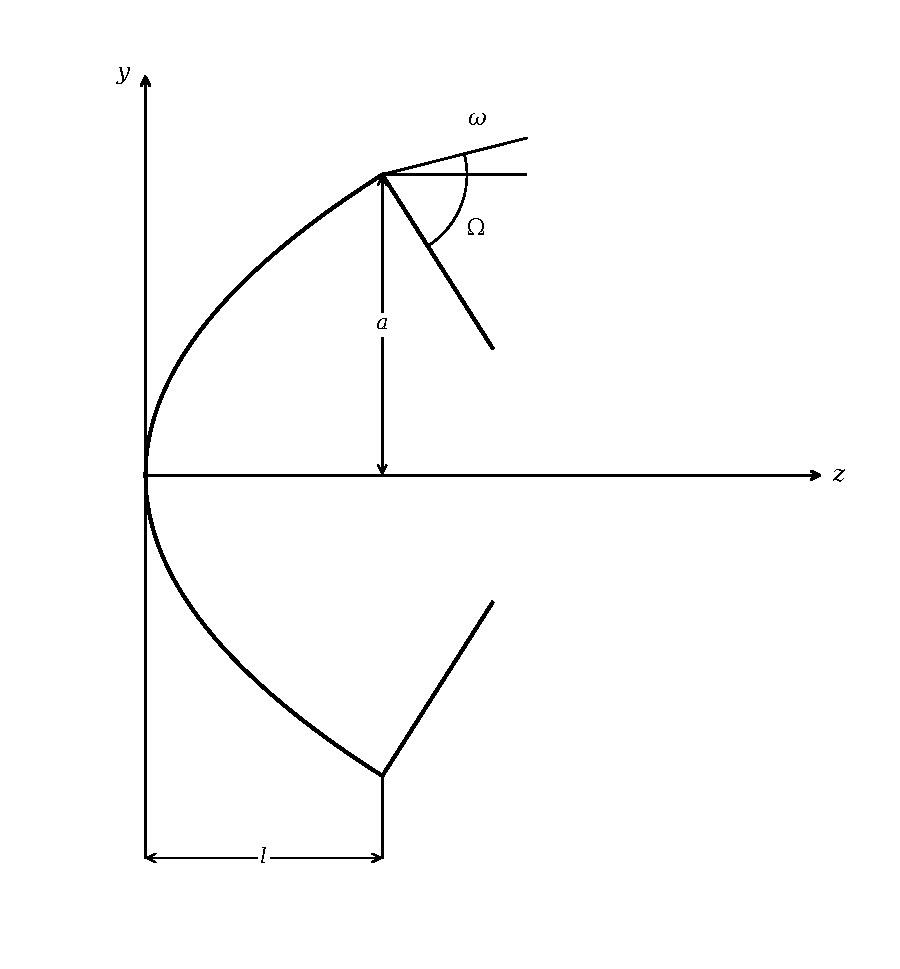
\includegraphics[width=.58\linewidth]{images/recreated/b-0126-fig42.pdf}

\raggedright Figure 42. A spherical segment with a conically shaped base.
\end{minipage}
\[\begin{aligned}E_x=-H_y=E_{0x}\left[-\frac a{2\cos\omega}+\frac i{4k}+\left(\frac a2\operatorname{tg}\omega-\frac i{4k}\right)e^{2ikl}\right]\frac{e^{ikR}}R.
\end{aligned}\tag{19.05}\]
Here we used the new designations
\[\left.\begin{aligned}a&=a_2,\quad\omega=\omega_2,\\l&=l_2=\rho(1-\sin\omega).\end{aligned}\right\}\tag{19.06}\]
Equations (19.02) and (19.05) are simplified if $ka_1\gg1$ and $ka_2\gg1$. Thus, the field from the spherical ring will equal
\[E_x=-H_y=-E_{0x}\left(\frac{a_1}2\operatorname{tg}\omega_1-\frac{a_2}2\operatorname{tg}\omega_2e^{2ikl_2}\right)e^{2ikl_1}\frac{e^{ikR}}R,\tag{19.07}\]
and the field from the spherical segment will equal
\[E_x=-H_y=-\frac{aE_{0x}}2(\sec\omega-\operatorname{tg}\omega\,e^{2ikl})\frac{e^{ikR}}R.\tag{19.08}\]
If here one assumes $\omega=0$, then equation
\[E_x=-H_y=-\frac{aE_{0x}}2\frac{e^{ikR}}R\tag{19.09}\]
gives us the field scattered by a hemisphere. The value of the effective scattering area corresponding to it will equal, in accordance with (17.06),
\[\sigma^0=\pi a^2.\tag{19.10}\]
\end{scanpage}
